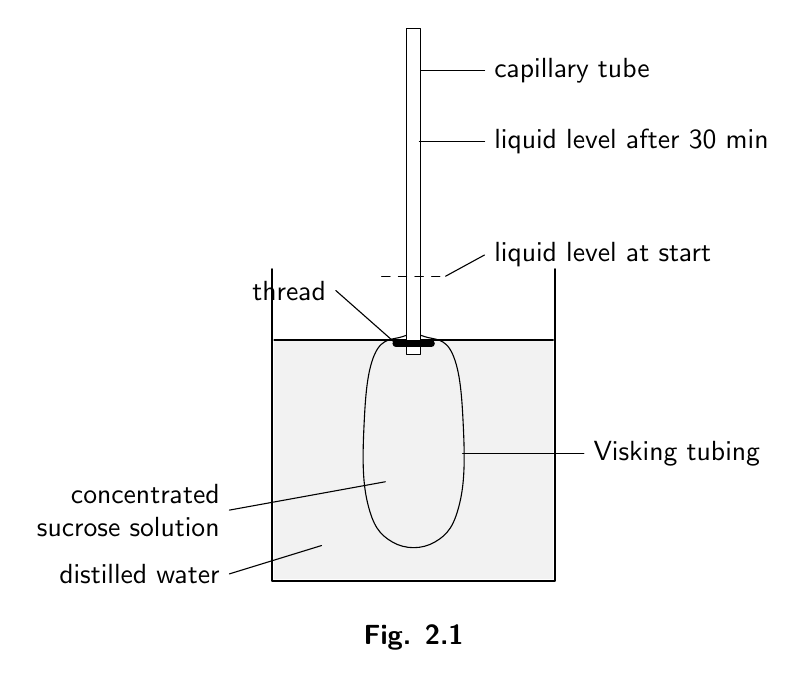
\begin{tikzpicture}[scale=0.9, font=\sffamily, line join=round, line cap=round]
  % distilled water in beaker
  \fill[gray!10] (0.03,0.03) rectangle (3.97,3.4);
  \draw (0.03,3.4)--(3.97,3.4);
  \draw[thick] (0,4.4)--(0,0)--(4,0)--(4,4.4);
  % Visking tubing bag with concentrated sucrose solution (dotted)
  \begin{scope}
    \clip plot[smooth cycle, tension=0.7] coordinates {(1.45,3.2) (1.3,2.2) (1.35,1.1) (1.7,0.55) (2.3,0.55) (2.65,1.1) (2.7,2.2) (2.55,3.2) (2.15,3.45) (1.85,3.45)};
    \dotregion{1.2}{0.4}{2.8}{3.6}
  \end{scope}
  \draw plot[smooth cycle, tension=0.7] coordinates {(1.45,3.2) (1.3,2.2) (1.35,1.1) (1.7,0.55) (2.3,0.55) (2.65,1.1) (2.7,2.2) (2.55,3.2) (2.15,3.45) (1.85,3.45)};
  % capillary tube with liquid risen to 6.2
  \draw[fill=white] (1.9,3.2) rectangle (2.1,7.8);
  \dotregion{1.92}{3.2}{2.08}{6.2}
  \draw[line width=2.5pt] (1.75,3.35)--(2.25,3.35);
  \draw[dashed] (1.55,4.3)--(2.45,4.3);
  % labels
  \draw (2.1,7.2)--(3.0,7.2) node[right] {capillary tube};
  \draw (2.08,6.2)--(3.0,6.2) node[right] {liquid level after 30 min};
  \draw (2.45,4.3)--(3.0,4.6) node[right] {liquid level at start};
  \draw (1.75,3.35)--(0.9,4.1) node[left] {thread};
  \draw (2.69,1.8)--(4.4,1.8) node[right] {Visking tubing};
  \draw (1.6,1.4)--(-0.6,1.0) node[left, align=right] {concentrated\\sucrose solution};
  \draw (0.7,0.5)--(-0.6,0.1) node[left] {distilled water};
  \node[font=\sffamily\bfseries] at (2,-0.8) {Fig. 2.1};
\end{tikzpicture}
